\documentclass[border=10pt]{standalone}
\usepackage{pgfplots}
\usepgfplotslibrary{colormaps}
\pgfplotsset{compat=1.18, trig format plots=rad}
\begin{document}
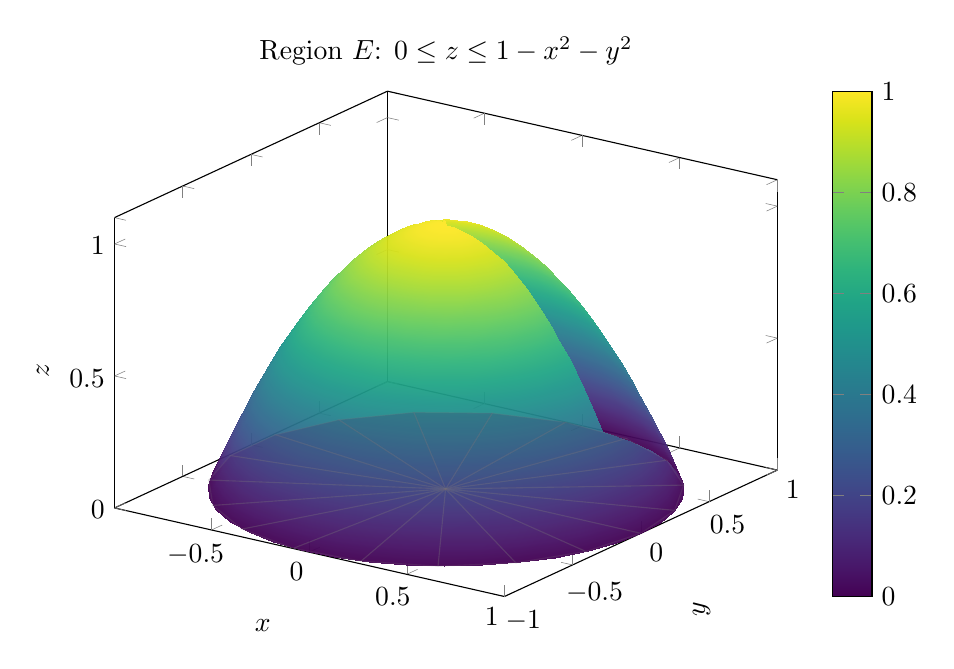
\begin{tikzpicture}
\begin{axis}[
    view={35}{28},
    width=10cm, height=8cm,
    xlabel={$x$}, ylabel={$y$}, zlabel={$z$},
    domain=0:1, y domain=0:2*pi,
    samples=25, samples y=40,
    variable=\r, variable y=\t,
    colormap/viridis,
    colorbar,
    point meta min=0, point meta max=1,
    zmin=0, zmax=1.1,
    axis lines=box,
    title={Region $E$: $0\le z\le 1-x^2-y^2$}
]
\addplot3[surf, shader=interp, opacity=0.95]
    ({r*cos(t)}, {r*sin(t)}, {1-r^2});
\addplot3[surf, opacity=0.18, faceted color=gray, samples=2, samples y=20]
    ({r*cos(t)}, {r*sin(t)}, {0});
\end{axis}
\end{tikzpicture}
\end{document}
